\section{Optimisation des hyper-paramètres et choix d'un modèle}\label{chapter-ML-section-hyperparameters}
Le choix d'un modèle et de ses hyper-paramètres est l'objet de cette section.
%Deux types de modèle sont étudiés:
%\begin{itemize}
%\item des arbres de décision améliorés, introduits section~\ref{chapter-ML-section-XGB}, notés XGB;
%\item des réseaux de neurones profonds, introduits section~\ref{chapter-ML-section-DNN}, notés DNN.
%\end{itemize}
Les hyper-paramètres des XGBs, introduits section~\ref{chapter-ML-section-XGB}, sont:
\begin{itemize}
\item la profondeur maximale des arbres \MaxDepth;
\item la quantité d'échantillons minimale dans une branche \MinChildWeight;
\item le nombre d'arbres \Nestimators;
\item le gain minimal $\gamma$;
\item le taux d'apprentissage $\eta$;
\item la fonction de coût \Loss;
\item la liste des variables d'entrée.
\end{itemize}
Les hyper-paramètres des DNNs, introduits section~\ref{chapter-ML-section-DNN}, sont:
\begin{itemize}
\item le nombre de couches cachées $N_L$;
\item le nombre de neurones par couche cachée $N_N$;
\item la fonction d'activation des neurones des couches cachées;
\item l'algorithme d'optimisation;
\item la fonction de coût \Loss;
\item le mode d'initiation des poids;
\item la liste des variables d'entrée.
\end{itemize}
\par
Les modèles entraînés ont pour but de prédire la masse générée du boson de Higgs $m_{\higgsML}$.
Une représentation graphique possible afin de montrer les performances d'un modèle est de représenter ses prédictions \ypred\ en fonction de \ytrue\ dans un histogramme à deux dimensions
comme sur la figure~\ref{subfig-pred_vs_ans_2d_histo_example}.
L'objectif des modèles est alors de se rapprocher autant que possible de la première bissectrice, tracée en rouge.
Toutefois
la large gamme explorée, de \num{50} à \SI{800}{\GeV}, rend difficile
la visualisation des performances à basse masse.
Or, cette région est importante car elle contient les bosons \Zboson\ et \higgs\ du modèle standard.
La réponse $r$ du modèle, définie comme
\begin{equation}
r = \frac{\ypred}{\ytrue} = \frac{F(\vec{x})}{m_{\higgsML}}
\mend[,]
\end{equation}
permet de ramener l'objectif des modèles à 1 sur toute la gamme de masse.
La réponse du même modèle est ainsi représentée sur la figure~\ref{subfig-model_response_example}.
Pour chaque intervalle de \SI{10}{\GeV} sur $m_{\higgsML}$,
la distribution de $r$ est déterminée.
La valeur moyenne et la médiane de cette distribution sont données,
et ainsi que le premier ($\pm1\sigma$) et le second quantile ($\pm2\sigma$).
Une évaluation quantifiée des modèles reste nécessaire.
\begin{figure}[h]
\centering

\subcaptionbox{Histogramme à deux dimensions de \ypred\ en fonction de \ytrue.\label{subfig-pred_vs_ans_2d_histo_example}}[.45\textwidth]
{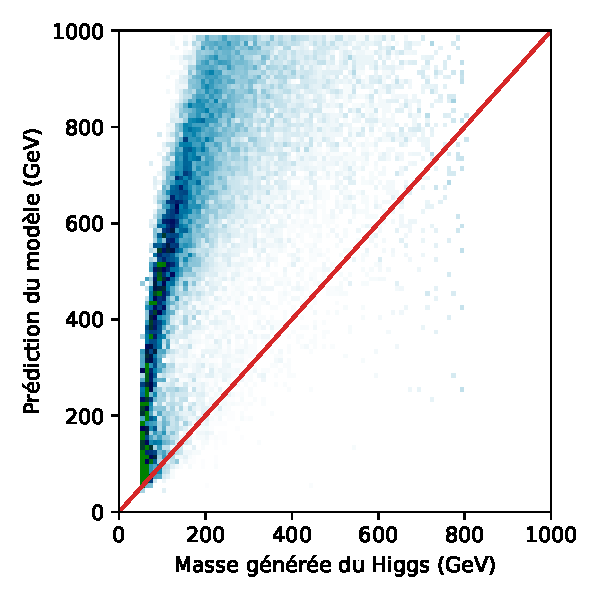
\includegraphics[width=.45\textwidth]{\PhDthesisdir/plots_and_images/my_plots/ML/from_ML_plots/trained_NNs_FastSim/DeepTau-inclusive/PuppiMET_with_METcov_j1j2jr_Nnu_Npu/predicted_vs_answers_histo-NN-ADAM_glorot_uniform-activation-softplus-batch_size-2048-mape-Adadelta-u-inclusive-3-layers-1000-neurons.pdf}}
\hfill
\subcaptionbox{Réponse du modèle $\ypred/\ytrue$ en fonction de \ytrue.\label{subfig-model_response_example}}[.45\textwidth]
{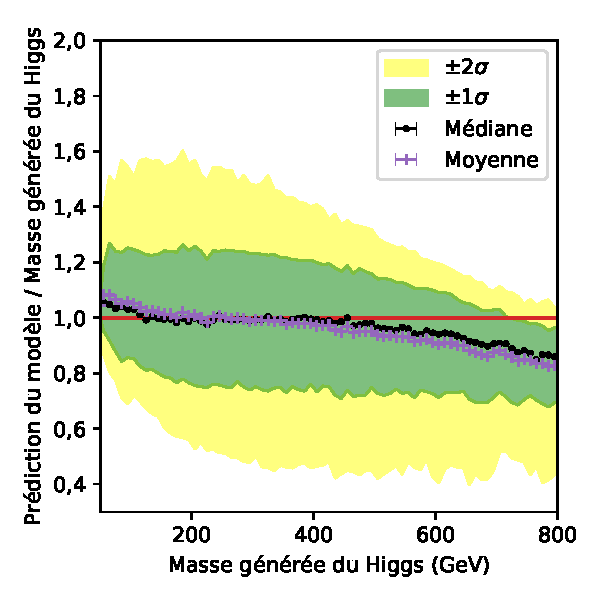
\includegraphics[width=.45\textwidth]{\PhDthesisdir/plots_and_images/my_plots/ML/from_ML_plots/trained_NNs_FastSim/DeepTau-inclusive/PuppiMET_with_METcov_j1j2jr_Nnu_Npu/model_response-NN-ADAM_glorot_uniform-activation-softplus-batch_size-2048-mape-Adadelta-u-inclusive-3-layers-1000-neurons.pdf}}

\caption{Exemples de graphiques rendant compte des performances des modèles.}
\label{fig-model_perfs_graphiques_examples}
\end{figure}
\par
Il est difficile de définir un seul score quantifiant la qualité d'un modèle.
Plusieurs métriques sont considérées afin d'évaluer les modèles:
\begin{itemize}
\item les valeurs de
\LossMSE,
\LossMAE,
\LossMAPE;
\item la résolution relative des modèles,
ou \og largeur à $1\sigma$ \fg,
notée \OneSigmaWidth,
estimée par
la moyenne
de
la largeur du premier quantile de la distribution de la réponse $r$ des modèles
sur des intervalles de \SI{10}{\GeV} sur $\ytrue=m_{\higgsML}$,
\ie
\begin{equation}
\OneSigmaWidth = \Average{\eval{\sigma\left(\frac{\ypred}{\ytrue}\right)}_{\ytrue\in [n, n+1]\times\SI{10}{\GeV}}}_n
\mend
\end{equation}
Il s'agit donc de la moyenne de la largeur verticale des bandes vertes ($\pm1\sigma$) sur les graphiques des réponses des modèles comme celui de la figure~\ref{subfig-model_response_example}.
\end{itemize}
Pour toutes ces métriques, l'objectif est la plus petite valeur possible.
De plus, quatre domaines de masse sont définis:
\begin{itemize}
\item basse masse : $m_{\higgsML} < \SI{150}{\GeV}$, incluant en particulier les bosons \Zboson\ et \higgs;
\item masse moyenne : $\SI{150}{\GeV} \leq m_{\higgsML} < \SI{500}{\GeV}$;
\item haute masse : $m_{\higgsML} \geq \SI{500}{\GeV}$;
\item toute masse : aucune restriction sur $m_{\higgsML}$.
\end{itemize}
Ils permettent de comparer les performances des modèles sur certaines gammes de masse uniquement.
Sauf contre-indication, toute la gamme de masse est considérée.
\par
Face à l'immense quantité de combinaisons différentes d'hyper-paramètres, toutes n'ont pas été créées.
Nous avons en revanche entraîné suffisamment de modèles afin d'observer les distributions des différentes métriques d'évaluation
pour des groupes de modèles ayant une valeur donnée d'un hyper-paramètre.
La comparaison des différentes distributions permet dans un premier temps de
voir quelles valeurs d'hyper-paramètres donnent des modèles moins performants
et ainsi se rapprocher d'une combinaison optimale,
comme l'exposent les sections~\ref{chapter-ML-section-hyperparameters-inputs} à~\ref{chapter-ML-section-hyperparameters-opti}.
Une fois certains hyper-paramètres fixés,
la sélection finale d'un seul modèle est réalisée selon la procédure
présentée en section~\ref{chapter-ML-section-hyperparameters-others}.
\subsection{Variables d'entrée}\label{chapter-ML-section-hyperparameters-inputs}
Les différentes variables d'entrée considérées sont listées dans la section~\ref{chapter-ML-section-evt_gen-inputs}.
La plupart de celles-ci sont généralement déjà exploitées dans les analyses en cours.
Ce n'est toutefois pas garanti, en particulier pour les variables relatives à l'activité hadronique additionnelle.
L'utilisation de variables supplémentaires demande,
en plus de la mise en place de leur obtention,
de reprendre potentiellement de longues étapes de calculs.
Se restreindre à un sous-ensemble des variables d'entrée,
si cela ne dégrade pas la qualité de nos modèles,
pourrait donc faciliter leur intégration dans des analyses.
\par
Les sous-ensembles des variables d'entrée sont définis par les restrictions suivantes:
\begin{itemize}
\item sans \Npu: la variable \Npu\ n'est pas utilisée;
\item sans \Nnu: la variable \Nnu\ n'est pas utilisée;
\item sans AHA: les variables d'activité hadronique additionnelle ne sont pas utilisées;
\item sans jets: les variables relatives aux jets (dont AHA) ne sont pas utilisées;
\item sans \mT: les masses transverses ne sont pas utilisées;
\item sans METcov: la matrice de covariance de \MET\ n'est pas utilisée.
\end{itemize}
L'application de plusieurs de ces restrictions est également testée.
\par
Les performances modèles entraînés avec les différents ensembles de variables d'entrée sont données
figure~\ref{fig-XGB_inputs} pour les XGBs
et
figure~\ref{fig-DNN_inputs}
pour les DNNs.
Les modèles concernés par plusieurs restrictions sont comptés de manière pondérée dans chaque groupe correspondant à une restriction unique.
Par exemple, un modèle soumis à la restriction \og sans \Npu\ \fg{} et \og sans \Nnu\ \fg{} a un poids de $\frac{1}{2}$ dans chacun de ces deux groupes.
Une pondération par la quantité de modèles dans chaque groupe est de plus appliquée pour supprimer le biais lié à la quantité accrue de modèles dans le groupe sans restrictions.
Les histogrammes ainsi créés sont superposés.
Il est alors possible de voir les contributions de chacune des restrictions aux valeurs obtenues sur la métrique d'évaluation illustrée.
\begin{figure}[h]
\centering

\subcaptionbox{Évaluation par \LossMAPE.\label{subfig-XGB_inputs-mape}}[.45\textwidth]
{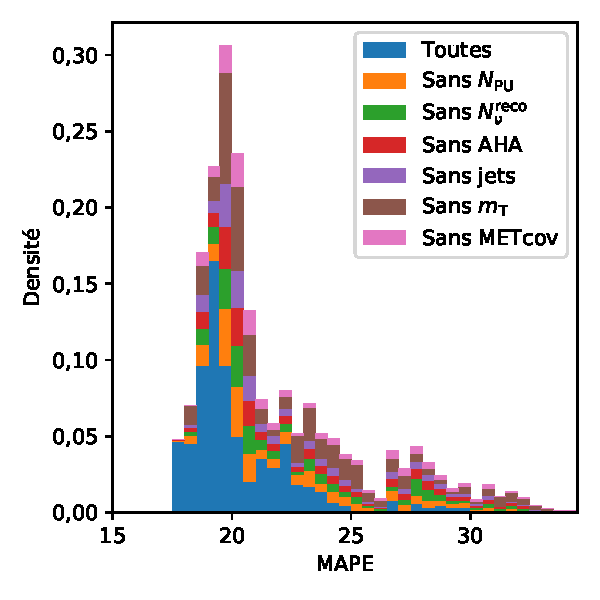
\includegraphics[width=.45\textwidth]{\PhDthesisdir/plots_and_images/my_plots/ML/from_ML_plots/global_comparisons/XGB_inputs_all-full_mape.pdf}\vspace{-\baselineskip}}
\hfill
\subcaptionbox{Évaluation par \OneSigmaWidth.\label{subfig-XGB_inputs-1sigw}}[.45\textwidth]
{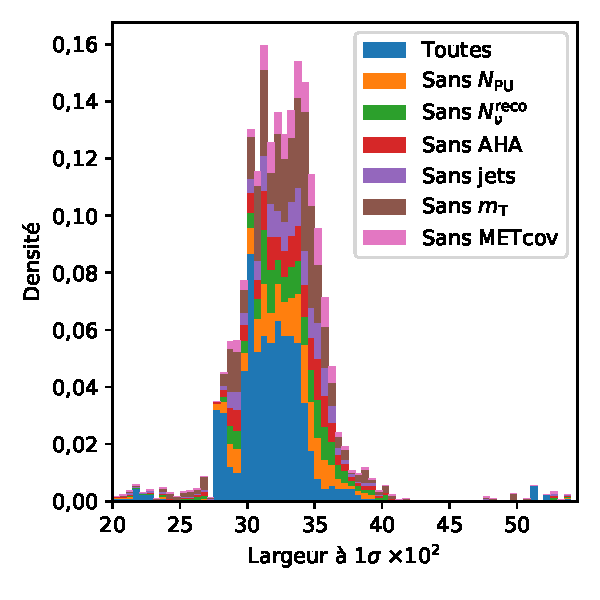
\includegraphics[width=.45\textwidth]{\PhDthesisdir/plots_and_images/my_plots/ML/from_ML_plots/global_comparisons/XGB_inputs_all-full_1sig_width.pdf}\vspace{-\baselineskip}}

\caption{Évaluations des XGBs regroupés selon les variables d'entrée.}
\label{fig-XGB_inputs}
\end{figure}
\begin{figure}[h]
\centering

\subcaptionbox{Évaluation par \LossMAPE.\label{subfig-DNN_inputs-mape}}[.45\textwidth]
{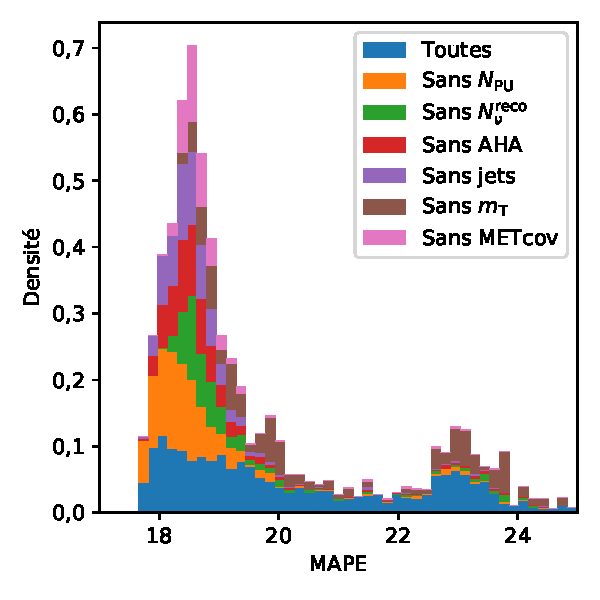
\includegraphics[width=.45\textwidth]{\PhDthesisdir/plots_and_images/my_plots/ML/from_ML_plots/global_comparisons/DNN_inputs_all-full_mape.pdf}\vspace{-\baselineskip}}
\hfill
\subcaptionbox{Évaluation par \OneSigmaWidth.\label{subfig-DNN_inputs-1sigw}}[.45\textwidth]
{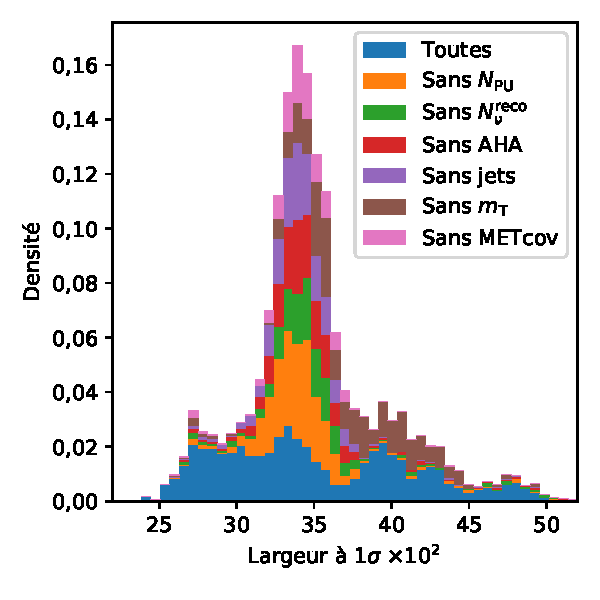
\includegraphics[width=.45\textwidth]{\PhDthesisdir/plots_and_images/my_plots/ML/from_ML_plots/global_comparisons/DNN_inputs_all-full_1sig_width.pdf}\vspace{-\baselineskip}}

\caption{Évaluations des DNNs regroupés selon les variables d'entrée.}
\label{fig-DNN_inputs}
\end{figure}
\par
Dans le cas des XGBs,
l'évaluation des modèles par \LossMAPE, en figure~\ref{subfig-XGB_inputs-mape},
donne des valeurs situées entre \num{17} et \num{35}.
Le cœur de la distribution,
à $\LossMAPE=\num{19}\pm\num{2}$,
est plutôt constitué
de modèles utilisant
toutes les entrées
dans sa partie gauche ($\LossMAPE<\num{19}$)
et
de modèles utilisant
un sous-ensemble d'entrées
dans sa partie droite ($\num{19}<\LossMAPE<\num{22}$).
De plus, les basses valeurs de \LossMAPE, en-dessous de \num{18.5},
sont presque exclusivement obtenues avec des modèles utilisant toutes les entrées.
À l'inverse, la queue à hautes valeurs de la distribution obtenue ($\LossMAPE>\num{23}$) est largement dominée par les contributions des modèles avec un sous-ensemble d'entrées.
\par
La plupart des XGBs ont
une largeur \OneSigmaWidth, en figure~\ref{subfig-XGB_inputs-1sigw},
située entre \num{27} et \num{38}.
Cependant,
les XGBs utilisant toutes les variables d'entrée
exhibent une distribution de \OneSigmaWidth\ légèrement décalée vers de plus faibles valeurs.
\par
Dans le cas des DNNs,
la distribution de la métrique \LossMAPE, en figure~\ref{subfig-DNN_inputs-mape},
contient des valeurs situées entre \num{17.5} et \num{25}.
Les DNNs n'utilisant pas \Nnu\
se situent à $\LossMAPE>\num{18}$.
Cette variable permet aux modèles de différencier les canaux
hadroniques, semi-leptoniques et leptoniques,
dont la séparation est discutée dans la section~\ref{chapter-ML-section-discussion}.
Ceux n'utilisant pas \mT\ présentent également des valeurs de \LossMAPE\ uniquement au-delà de \num{18}.
L'utilisation de ces variables permet donc d'obtenir de meilleurs modèles.
Elles sont de plus facilement obtenues à partir du \emph{dilepton}, défini chapitre~\refChHTT, et de \MET.
Les analyses avec deux leptons tau dans l'état final exploitent déjà ces observables,
leur utilisation par nos modèles est donc à la fois
pertinente, car les scores de \LossMAPE\ obtenus sont meilleurs,
et
sans incidence sur la facilité d'intégration du modèle à l'analyse.
Les DNNs avec $\LossMAPE\lesssim\num{18}$
exploitent presque tous
les variables relatives aux jets, à l'AHA et à la matrice de covariance de \MET.
Ces entrées sont donc vraisemblablement utiles aux DNNs afin de réaliser la régression.
Enfin,
la restriction sur \Npu\
ne semble pas dégrader les performances des DNNs
selon \LossMAPE.
\par
La distribution de
\OneSigmaWidth, en figure~\ref{subfig-DNN_inputs-1sigw},
montre que les modèles utilisant toutes les entrées peuvent se répartir en plusieurs groupes,
aux alentour des valeurs
\num{0.275}, \num{0.335}, \num{0.395}, \num{0.425} et \num{0.475}.
À \num{0.395} apparaît également un groupe de modèles entraînés sans \mT.
À \num{0.335} se trouvent la majorité des modèles entraînés avec une restriction des entrées.
%Les modèles de ces groupes ont potentiellement minimisé l'utilisation de certaines variables.
%Les modèles d'intérêt sont ceux du groupe se situant à $\OneSigmaWidth \simeq \num{0.275}$.
%Il s'agit presque exclusivement de modèles utilisant toutes les variables d'entrée.
Pour $\OneSigmaWidth<\num{0.3}$, les modèles sont très majoritairement ceux utilisant l'ensemble des variables proposées.
\par
L'utilisation de toutes les variables listées dans la section~\ref{chapter-ML-section-evt_gen-inputs}
est donc corrélée avec de meilleures performances
selon les métriques
\LossMAPE\
et
\OneSigmaWidth.
Par la suite, seuls les modèles utilisant toutes les variables, au nombre de 27, sont considérés.
\subsection{Type de modèle}\label{chapter-ML-section-hyperparameters-type}
Les figures~\ref{fig-DNN_vs_XGB-mse_mape} et~\ref{fig-DNN_vs_XGB-1sigma}
présentent les distributions des scores de
\LossMSE,
\LossMAPE\
et
\OneSigmaWidth\
pour l'ensemble des DNNs et des XGBs
utilisant toutes les variables d'entrée.
\par
\begin{figure}[h]
\centering

\subcaptionbox{Évaluation par \LossMSE.\label{subfig-DNN_vs_XGB-mse}}[.45\textwidth]
{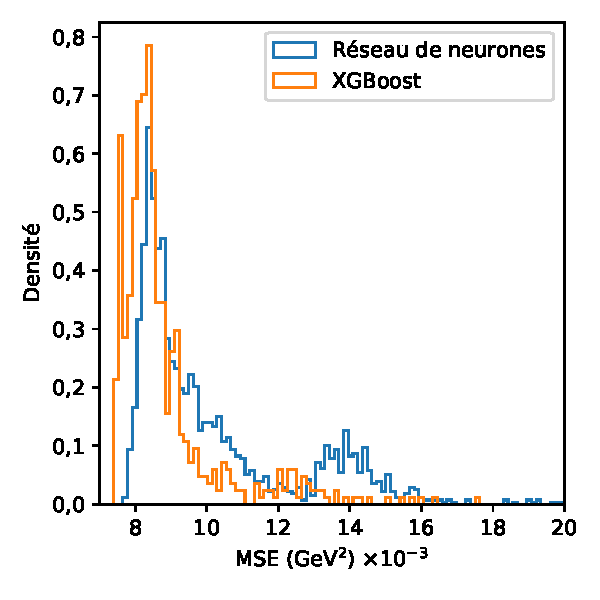
\includegraphics[width=.45\textwidth]{\PhDthesisdir/plots_and_images/my_plots/ML/from_ML_plots/global_comparisons/DNN_vs_XGB_all_inputs-full_mse.pdf}\vspace{-\baselineskip}}
\hfill
\subcaptionbox{Évaluation par \LossMAPE.\label{subfig-DNN_vs_XGB-mape}}[.45\textwidth]
{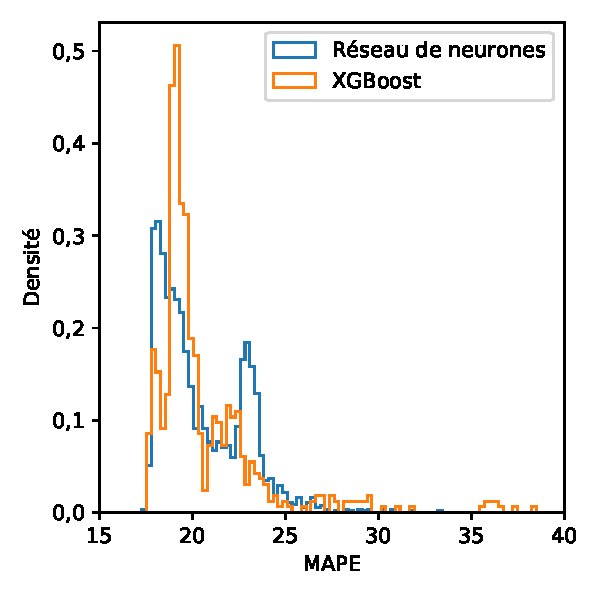
\includegraphics[width=.45\textwidth]{\PhDthesisdir/plots_and_images/my_plots/ML/from_ML_plots/global_comparisons/DNN_vs_XGB_all_inputs-full_mape.pdf}\vspace{-\baselineskip}}

\caption{Évaluations des XGBs et des DNNs par \LossMSE\ et \LossMAPE.}
\label{fig-DNN_vs_XGB-mse_mape}
\end{figure}
\begin{figure}[h]
\centering
%\vspace{\baselineskip}

%\subcaptionbox{\label{subfig-DNN_vs_XGB-mae}}[.45\textwidth]
%{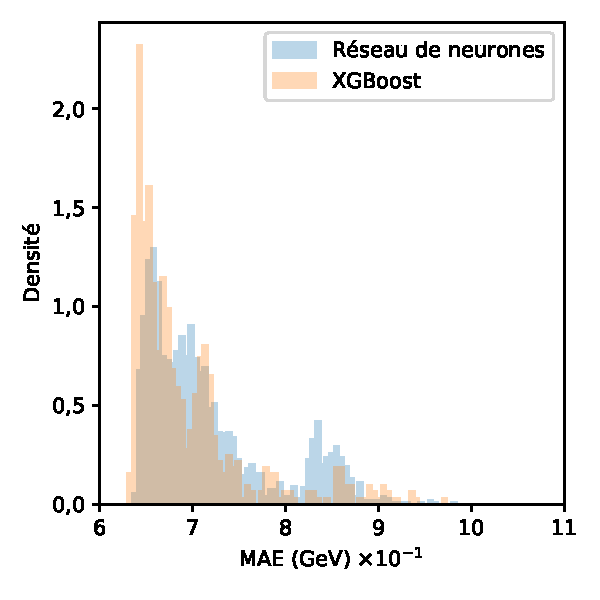
\includegraphics[width=.45\textwidth]{\PhDthesisdir/plots_and_images/my_plots/ML/from_ML_plots/global_comparisons/DNN_vs_XGB_all_inputs-full_mae.pdf}\vspace{-\baselineskip}}
%\hfill
\subcaptionbox{Sur toute la gamme de masse.\label{subfig-DNN_vs_XGB-1sigma}}[.45\textwidth]
{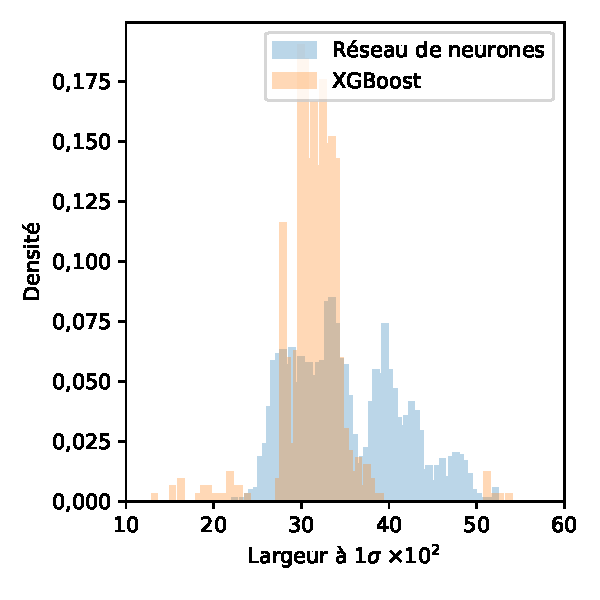
\includegraphics[width=.45\textwidth]{\PhDthesisdir/plots_and_images/my_plots/ML/from_ML_plots/global_comparisons/DNN_vs_XGB_all_inputs-full_1sig_width.pdf}\vspace{-\baselineskip}}
\hfill
\subcaptionbox{À basse masse.\label{subfig-DNN_vs_XGB-low_1sigma}}[.45\textwidth]
{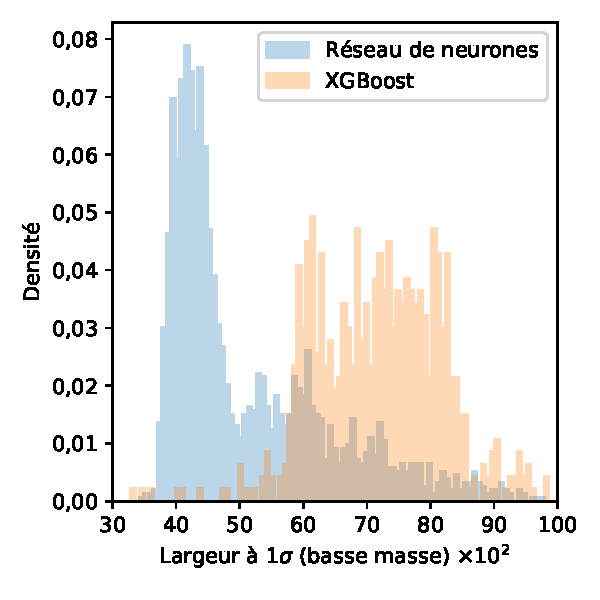
\includegraphics[width=.45\textwidth]{\PhDthesisdir/plots_and_images/my_plots/ML/from_ML_plots/global_comparisons/DNN_vs_XGB_all_inputs-low_1sig_width.pdf}\vspace{-\baselineskip}}

\caption{Évaluations des XGBs et des DNNs par \OneSigmaWidth.}
\label{fig-DNN_vs_XGB-1sigma}
\end{figure}
L'évaluation par \LossMSE, en figure~\ref{subfig-DNN_vs_XGB-mse}, favorise les XGBs.
Le cœur de la distribution de \LossMSE\ pour ces modèles est en effet à \SI{8.1e3}{\GeV^2}
contre \SI{8.5e3}{\GeV^2} pour les DNNs.
En revanche,
l'évaluation par \LossMAPE, en figure~\ref{subfig-DNN_vs_XGB-mape}, favorise les DNNs
avec un groupe de DNNs à $\LossMAPE=\num{18}$
contre \num{19} pour les XGBs.
Un second groupe de DNNs est présent à $\LossMAPE=\num{23}$.
L'existence de ces deux groupes est due à l'utilisation de plusieurs algorithmes d'optimisation, comme discuté dans la section~\ref{chapter-ML-section-hyperparameters-opti}.
\par
La résolution des modèles est évaluée par \OneSigmaWidth\
en figure~\ref{subfig-DNN_vs_XGB-1sigma} pour toute la gamme de masse
et
en figure~\ref{subfig-DNN_vs_XGB-low_1sigma} pour les basses masses.
Sur l'ensemble de la gamme de masse,
les XGBs ont un score de $\num{0.32}\pm\num{0.04}$
et
les DNNs se répartissent en plusieurs groupes
à environ
\num{0.28}, \num{0.33}, \num{0.40}, \num{0.42} et \num{0.48}.
%\num{0.275}, \num{0.335}, \num{0.395}, \num{0.425} et \num{0.475}.
Les XGBs sont ainsi compétitifs d'après cette évaluation.
Cependant,
les performances des modèles
à basse masse, \ie\ pour $m_{\higgsML} < \SI{150}{\GeV}$,
sont importantes car c'est dans cette gamme de masse que se trouvent les bosons \Zboson\ et \higgs\ du modèle standard.
Sur la figure~\ref{subfig-DNN_vs_XGB-low_1sigma},
l'évaluation à basse masse par \OneSigmaWidth\
les XGBs ont un score de $\num{0.70}\pm\num{0.15}$
alors que les DNNs se répartissent en deux groupes,
le premier à $\num{0.42}\pm\num{0.05}$
et
le second entre $\num{0.50}$ et $\num{1.0}$.
Le premier ensemble de DNNs propose les meilleures résolutions sur les masses des particules du modèle standard.
\par
La réévaluation des modèles par 
\LossMSE\ et \LossMAPE\ à basse masse, en figures~\ref{subfig-DNN_vs_XGB-low_mse} et~\ref{subfig-DNN_vs_XGB-low_mape},
confirme l'obtention de meilleures performances avec les DNNs.
En effet,
les DNNs sont les seuls modèles avec
$\LossMSE < \SI{1.5e3}{\GeV^2}$
et
$\LossMAPE < \num{28}$
à basse masse.
Les XGBs ont des scores de \LossMSE\ et \LossMAPE\ généralement
entre \SI{1.5e3}{\GeV^2} et \SI{4.0e3}{\GeV^2}
et
entre \num{28} et \num{43},
respectivement.
La suite de la sélection d'un modèle est donc faite parmi les DNNs.
\begin{figure}[h]
\centering
%\vspace{\baselineskip}

\subcaptionbox{Évaluation par \LossMSE.\label{subfig-DNN_vs_XGB-low_mse}}[.45\textwidth]
{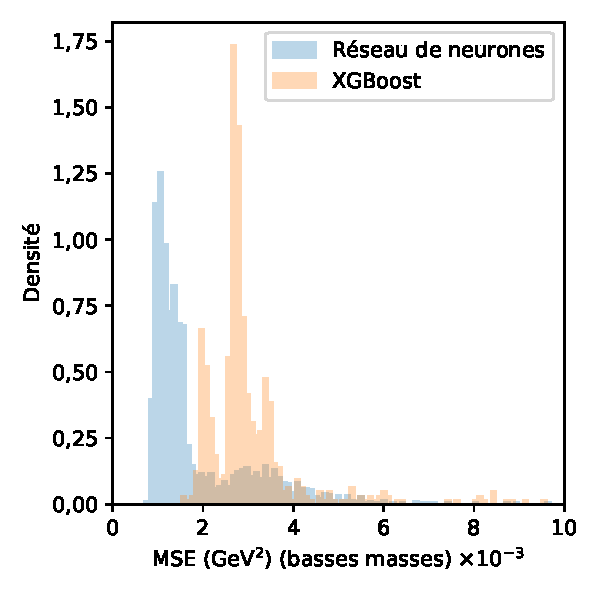
\includegraphics[width=.45\textwidth]{\PhDthesisdir/plots_and_images/my_plots/ML/from_ML_plots/global_comparisons/DNN_vs_XGB_all_inputs-low_mse.pdf}\vspace{-\baselineskip}}
\hfill
\subcaptionbox{Évaluation par \LossMAPE.\label{subfig-DNN_vs_XGB-low_mape}}[.45\textwidth]
{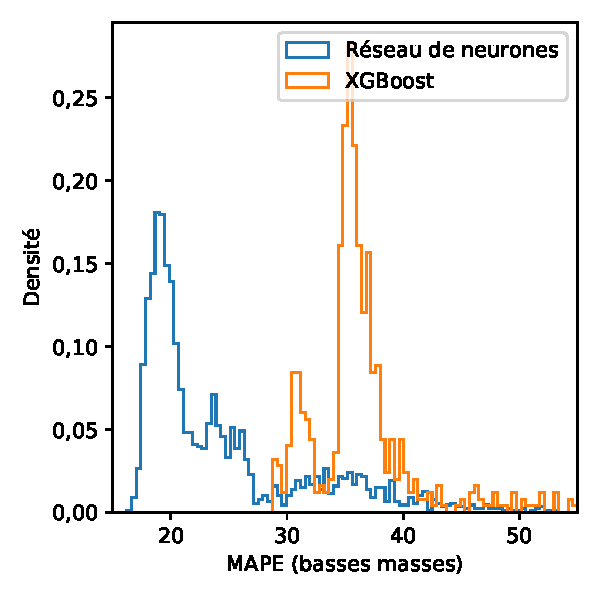
\includegraphics[width=.45\textwidth]{\PhDthesisdir/plots_and_images/my_plots/ML/from_ML_plots/global_comparisons/DNN_vs_XGB_all_inputs-low_mape.pdf}\vspace{-\baselineskip}}

\caption{Évaluations des XGBs et des DNNs par \LossMSE\ et \LossMAPE\ à basse masse.}
\label{fig-DNN_vs_XGB-mse_mape-low}
\end{figure}
\subsection{Fonction de coût}\label{chapter-ML-section-hyperparameters-loss}
Les évaluations des DNNs,
regroupés d'après la fonction de coût utilisée lors de leurs entraînements,
selon les métriques
\LossMSE, \LossMAPE, \LossMAE\ sur toute la gamme de masse et \OneSigmaWidth\ à basse masse
sont représentées sur la figure~\ref{fig-DNN_losses}.
\begin{figure}[h]
\centering

\subcaptionbox{\label{subfig-loss-mse}}[.45\textwidth]
{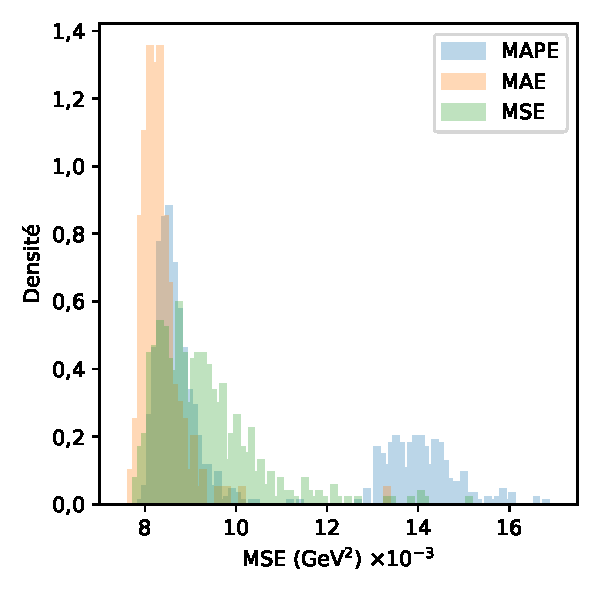
\includegraphics[width=.45\textwidth]{\PhDthesisdir/plots_and_images/my_plots/ML/from_ML_plots/global_comparisons/DNN_loss-full_mse.pdf}\vspace{-\baselineskip}}
\hfill
\subcaptionbox{\label{subfig-loss-mape}}[.45\textwidth]
{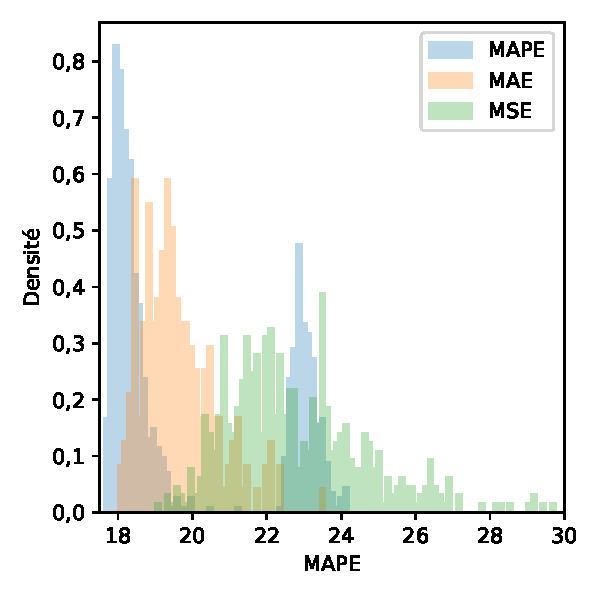
\includegraphics[width=.45\textwidth]{\PhDthesisdir/plots_and_images/my_plots/ML/from_ML_plots/global_comparisons/DNN_loss-full_mape.pdf}\vspace{-\baselineskip}}

\vspace{\baselineskip}

\subcaptionbox{\label{subfig-loss-mae}}[.45\textwidth]
{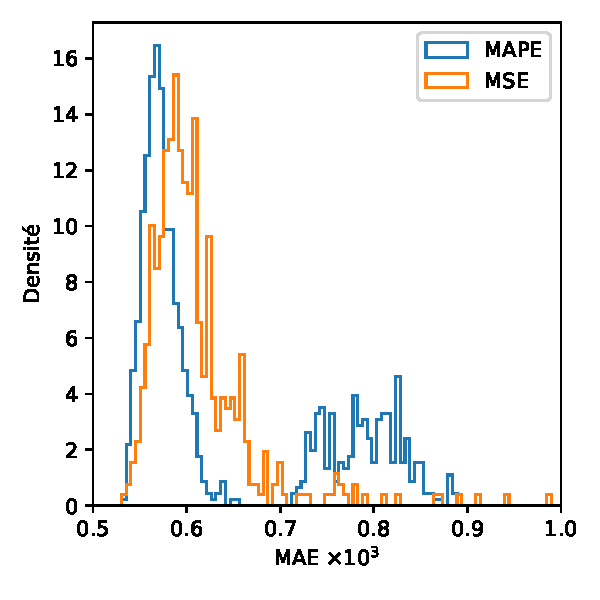
\includegraphics[width=.45\textwidth]{\PhDthesisdir/plots_and_images/my_plots/ML/from_ML_plots/global_comparisons/DNN_loss-full_mae.pdf}\vspace{-\baselineskip}}
\hfill
\subcaptionbox{\label{subfig-loss-low_1sigma}}[.45\textwidth]
{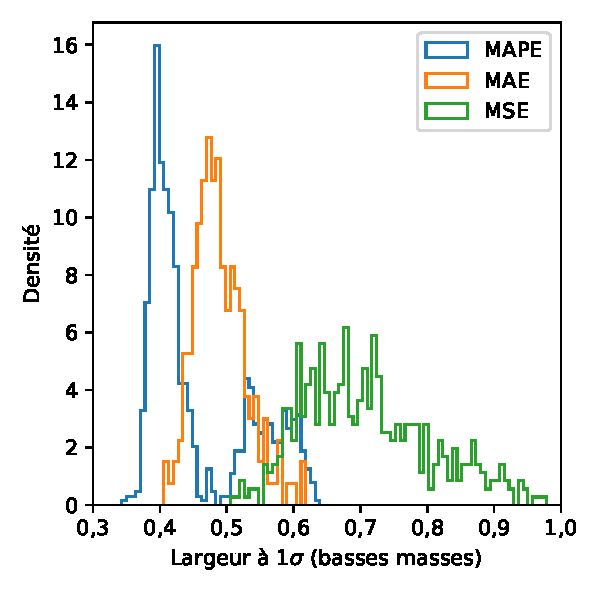
\includegraphics[width=.45\textwidth]{\PhDthesisdir/plots_and_images/my_plots/ML/from_ML_plots/global_comparisons/DNN_loss-low_1sig_width.pdf}\vspace{-\baselineskip}}

\caption{Évaluations des DNNs regroupés selon la fonction de coût par \LossMSE, \LossMAPE, \LossMAE\ et \OneSigmaWidth.}
\label{fig-DNN_losses}
\end{figure}
\par
L'évaluation par \LossMSE\ est représentée figure~\ref{subfig-loss-mse}.
Les DNNs entraînés avec $\Loss=\LossMSE$
y présentent un score
compris entre \SI{7.8e3}{\GeV^2} et \SI{15e3}{\GeV^2},
la majorité d'entre eux se trouvant en-dessous de \SI{11e3}{\GeV^2}
avec un pic de leur distribution à \SI{8.7e3}{\GeV^2}.
Les DNNs entraînés avec $\Loss=\LossMAE$
se situent majoritairement
entre \SI{7.7e3}{\GeV^2} et \SI{10e3}{\GeV^2},
avec un pic de leur distribution à \SI{8.3e3}{\GeV^2}.
Les DNNs entraînés avec $\Loss=\LossMAPE$
se répartissent en deux groupes,
le premier
entre \SI{7.9e3}{\GeV^2} et \SI{10e3}{\GeV^2},
le second
entre \SI{13e3}{\GeV^2} et \SI{16e3}{\GeV^2}.
La fonction de coût \LossMAE\ semble ainsi préférable à \LossMSE\ lorsque la comparaison de fait sur \LossMSE\ elle-même.
Il est en revanche plus difficile de conclure quant à \LossMAPE.
\par
L'évaluation par \LossMAPE, figure~\ref{subfig-loss-mape},
montre également un avantage de \LossMAE\ sur \LossMSE.
En effet, les modèles
entraînés avec $\Loss=\LossMAE$
se situent majoritairement à $\LossMAPE<\num{21}$
alors que ceux
entraînés avec $\Loss=\LossMSE$
sont plutôt dans la région $\LossMAPE>\num{20}$.
Les valeurs les plus basses sont obtenues sur les modèles entraînés avec \LossMAPE.
Or, l'évaluation est basée sur \LossMAPE\ elle-même,
il n'est donc pas équitable de se baser uniquement sur la figure~\ref{subfig-loss-mape}
pour affirmer que \LossMAPE\ peut être préférable à \LossMAE\ ou \LossMSE.
\par
La figure~\ref{subfig-loss-mae} représente l'évaluation des DNNs par \LossMAE.
La distribution obtenue avec les DNNs entraînés avec $\Loss=\LossMSE$
s'étend de \SI{65}{\GeV} à près de \SI{10}{\GeV} avec un pic à \SI{71}{\GeV}.
En revanche, de nombreux modèles entraînés avec \LossMAE\ ou \LossMAPE\
se situent à $\num{67}\pm\SI{4}{\GeV}$.
\par
Enfin,
sur la figure~\ref{subfig-loss-low_1sigma} se trouvent les distributions
de \OneSigmaWidth\ à basse masse pour ces trois groupes de DNNs.
Les modèles utilisant \LossMSE\ ont tous un score supérieur à \num{0.5}.
Ceux entraînés avec \LossMAE\ se situent entre \num{0.4} et \num{0.6}.
Les modèles basés sur \LossMAPE\ forment encore deux groupes,
le premier entre \num{0.34} et \num{0.5},
le second entre \num{0.5} et \num{0.64}.
Les fonctions de coût \LossMAPE\ et \LossMAE\ permettent donc d'obtenir des modèles avec une meilleure résolution à basse masse que \LossMSE.
\par
Les modèles entraînés avec $\Loss=\LossMAE$ ou $\Loss=\LossMAPE$
proposent de meilleurs scores que ceux obtenus avec $\Loss=\LossMSE$,
quelle que soit la métrique d'évaluation utilisée.
Lors des évaluations avec \LossMSE\ ou \LossMAE,
aucun avantage net n'est visible entre $\Loss=\LossMAE$ et $\Loss=\LossMAPE$.
En revanche, les métriques \LossMAPE\ et \OneSigmaWidth\ montrent que certains modèles
entraînés avec $\Loss=\LossMAPE$
donnent de meilleurs résultats.
La sélection d'un modèle est donc réalisée parmi ceux ayant comme fonction de coût \LossMAPE.
\subsection{Algorithme d'optimisation}\label{chapter-ML-section-hyperparameters-opti}
Les algorithmes d'optimisation sont présentés dans la section~\ref{chapter-ML-section-DNN-training-optimizers}.
L'algorithme SGD ne permet pas aux modèles de converger, il est donc exclu de nos investigations.
Deux algorithmes sont comparés, AdaDelta et Adam.
\par
Les évaluations des DNNs précédemment sélectionnés,
regroupés d'après l'algorithme d'optimisation utilisé lors de leurs entraînements,
selon les métriques
\LossMAPE\ sur toute la gamme de masse et \OneSigmaWidth\ à basse masse
sont représentées sur la figure~\ref{fig-optimizer}.
Les deux groupes observés dans les sections précédentes sont identifiés comme étant les modèles entraînés respectivement par Adam et AdaDelta.
Dans le cadre de nos travaux, lors de la recherche de la combinaison optimale d'hyper-paramètres,
nous avons initialement utilisé Adam jusqu'à sélectionner
le jeu de variables d'entrée (section~\ref{chapter-ML-section-hyperparameters-inputs})
et
la fonction de coût (section~\ref{chapter-ML-section-hyperparameters-loss}) à utiliser.
C'est pourquoi ces deux groupes liés à Adam et AdaDelta n'apparaissent que dans certaines sélections de modèles.
\begin{figure}[h]
\centering

\subcaptionbox{\label{subfig-optimizer-mape}}[.45\textwidth]
{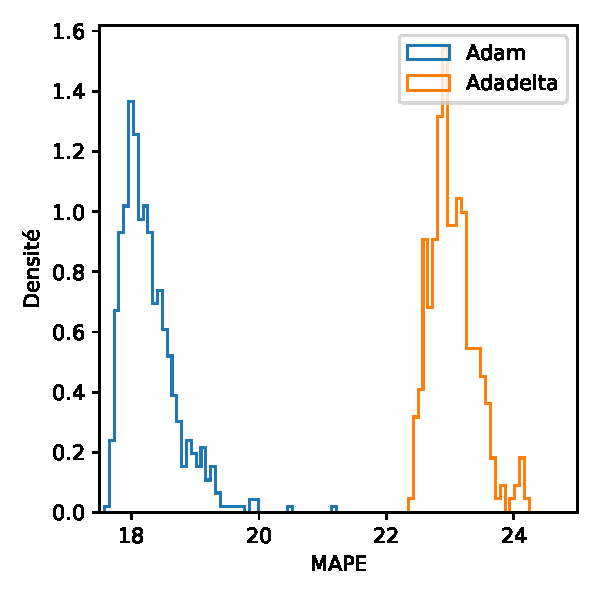
\includegraphics[width=.45\textwidth]{\PhDthesisdir/plots_and_images/my_plots/ML/from_ML_plots/global_comparisons/DNN_optimizer-full_mape.pdf}\vspace{-\baselineskip}}
\hfill
\subcaptionbox{\label{subfig-optimizer-low_1sigma}}[.45\textwidth]
{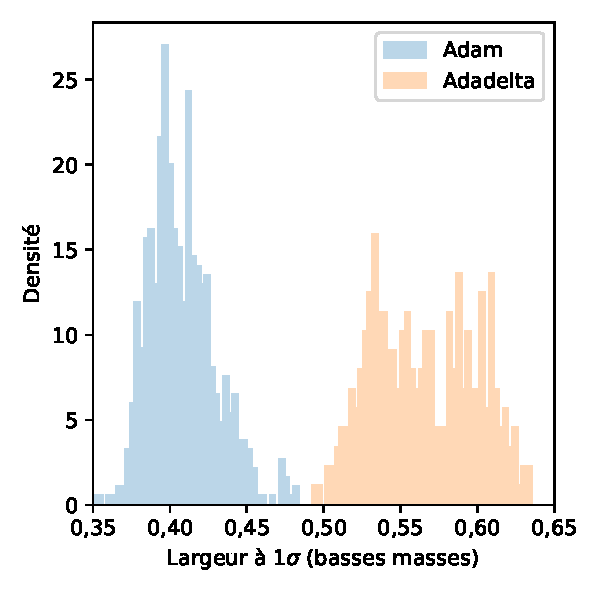
\includegraphics[width=.45\textwidth]{\PhDthesisdir/plots_and_images/my_plots/ML/from_ML_plots/global_comparisons/DNN_optimizer-low_1sig_width.pdf}\vspace{-\baselineskip}}

\caption{Évaluations des DNNs regroupés selon l'algorithme d'optimisation par \LossMAPE\ et \OneSigmaWidth.}
\label{fig-optimizer}
\end{figure}
\par
Sur la figure~\ref{subfig-optimizer-mape},
les modèles optimisés par Adam présentent un score de \LossMAPE\
entre \num{17.5} et \num{20}
alors que ceux optimisés par AdaDelta se situent
entre \num{22.2} et \num{24.3}.
L'optimisation par Adam semble donc meilleure que celle par AdaDelta.
L'évaluation à basse masse par \OneSigmaWidth\ sur la figure~\ref{subfig-optimizer-low_1sigma}
confirme cette observation.
Les modèles optimisés par Adam se situent en effet
entre \num{0.35} et \num{0.48},
ceux optimisés par AdaDelta
entre \num{0.49} et \num{0.64}.
\par
L'algorithme d'optimisation Adam donne de meilleurs modèles qu'AdaDelta.
\subsection{Autres hyper-paramètres}\label{chapter-ML-section-hyperparameters-others}
Les hyper-paramètres restant à être fixés ainsi que les valeurs explorées sont:
\begin{itemize}
\item le nombre de couches cachées $N_L$, 2 à 5;
\item le nombre de neurones par couche cachée $N_N$, \num{200} à \num{2000} par pas de \num{100};
\item le mode d'initiation des poids (WI), uniforme (u), normale (n), Glorot uniforme (gu), Glorot normale (gn);
\item la fonction d'activation (FA) des neurones des couches cachées, ReLU, SELU, ELU, Softplus.
\end{itemize}
Les évaluations
à basse, moyenne et haute masse
des DNNs
utilisant les 27 variables d'entrée
et
entraînés par Adam avec $\Loss=\LossMAPE$,
regroupés respectivement par
$N_L$, $N_N$, mode d'initiation des poids et fonction d'activation
sont données sur les
figures~\ref{fig-N_layers}, \ref{fig-N_neurons}, \ref{fig-w_init_mode} et~\ref{fig-activation} respectivement.
La position du modèle final sélectionné est également indiquée.
\def\localHP{N_layers}
\def\localHPlong{$N_L$}
\begin{figure}[p]
\centering

\subcaptionbox{\label{subfig-\localHP-low_mape}}[.45\textwidth]
{\includegraphics[width=.45\textwidth]{\PhDthesisdir/plots_and_images/my_plots/ML/from_ML_plots/global_comparisons/DNN_\localHP-low_mape.pdf}\vspace{-\baselineskip}}
\hfill
\subcaptionbox{\label{subfig-\localHP-low_1sigma}}[.45\textwidth]
{\includegraphics[width=.45\textwidth]{\PhDthesisdir/plots_and_images/my_plots/ML/from_ML_plots/global_comparisons/DNN_\localHP-low_1sig_width.pdf}\vspace{-\baselineskip}}

\subcaptionbox{\label{subfig-\localHP-medium_mape}}[.45\textwidth]
{\includegraphics[width=.45\textwidth]{\PhDthesisdir/plots_and_images/my_plots/ML/from_ML_plots/global_comparisons/DNN_\localHP-medium_mape.pdf}\vspace{-\baselineskip}}
\hfill
\subcaptionbox{\label{subfig-\localHP-medium_1sigma}}[.45\textwidth]
{\includegraphics[width=.45\textwidth]{\PhDthesisdir/plots_and_images/my_plots/ML/from_ML_plots/global_comparisons/DNN_\localHP-medium_1sig_width.pdf}\vspace{-\baselineskip}}

\subcaptionbox{\label{subfig-\localHP-high_mape}}[.45\textwidth]
{\includegraphics[width=.45\textwidth]{\PhDthesisdir/plots_and_images/my_plots/ML/from_ML_plots/global_comparisons/DNN_\localHP-high_mape.pdf}\vspace{-\baselineskip}}
\hfill
\subcaptionbox{\label{subfig-\localHP-high_1sigma}}[.45\textwidth]
{\includegraphics[width=.45\textwidth]{\PhDthesisdir/plots_and_images/my_plots/ML/from_ML_plots/global_comparisons/DNN_\localHP-high_1sig_width.pdf}\vspace{-\baselineskip}}

\caption{Évaluations des DNNs regroupés selon \localHPlong\ par \LossMAPE\ et \OneSigmaWidth.}
\label{fig-\localHP}
\end{figure}

\def\localHP{N_neurons}
\def\localHPlong{$N_N$}
\begin{figure}[p]
\centering

\subcaptionbox{\label{subfig-\localHP-low_mape}}[.45\textwidth]
{\includegraphics[width=.45\textwidth]{\PhDthesisdir/plots_and_images/my_plots/ML/from_ML_plots/global_comparisons/DNN_\localHP-low_mape.pdf}\vspace{-\baselineskip}}
\hfill
\subcaptionbox{\label{subfig-\localHP-low_1sigma}}[.45\textwidth]
{\includegraphics[width=.45\textwidth]{\PhDthesisdir/plots_and_images/my_plots/ML/from_ML_plots/global_comparisons/DNN_\localHP-low_1sig_width.pdf}\vspace{-\baselineskip}}

\subcaptionbox{\label{subfig-\localHP-medium_mape}}[.45\textwidth]
{\includegraphics[width=.45\textwidth]{\PhDthesisdir/plots_and_images/my_plots/ML/from_ML_plots/global_comparisons/DNN_\localHP-medium_mape.pdf}\vspace{-\baselineskip}}
\hfill
\subcaptionbox{\label{subfig-\localHP-medium_1sigma}}[.45\textwidth]
{\includegraphics[width=.45\textwidth]{\PhDthesisdir/plots_and_images/my_plots/ML/from_ML_plots/global_comparisons/DNN_\localHP-medium_1sig_width.pdf}\vspace{-\baselineskip}}

\subcaptionbox{\label{subfig-\localHP-high_mape}}[.45\textwidth]
{\includegraphics[width=.45\textwidth]{\PhDthesisdir/plots_and_images/my_plots/ML/from_ML_plots/global_comparisons/DNN_\localHP-high_mape.pdf}\vspace{-\baselineskip}}
\hfill
\subcaptionbox{\label{subfig-\localHP-high_1sigma}}[.45\textwidth]
{\includegraphics[width=.45\textwidth]{\PhDthesisdir/plots_and_images/my_plots/ML/from_ML_plots/global_comparisons/DNN_\localHP-high_1sig_width.pdf}\vspace{-\baselineskip}}

\caption{Évaluations des DNNs regroupés selon \localHPlong\ par \LossMAPE\ et \OneSigmaWidth.}
\label{fig-\localHP}
\end{figure}

\def\localHP{w_init_mode}
\def\localHPlong{le mode d'initiation des poids}
\begin{figure}[p]
\centering

\subcaptionbox{\label{subfig-\localHP-low_mape}}[.45\textwidth]
{\includegraphics[width=.45\textwidth]{\PhDthesisdir/plots_and_images/my_plots/ML/from_ML_plots/global_comparisons/DNN_\localHP-low_mape.pdf}\vspace{-\baselineskip}}
\hfill
\subcaptionbox{\label{subfig-\localHP-low_1sigma}}[.45\textwidth]
{\includegraphics[width=.45\textwidth]{\PhDthesisdir/plots_and_images/my_plots/ML/from_ML_plots/global_comparisons/DNN_\localHP-low_1sig_width.pdf}\vspace{-\baselineskip}}

\subcaptionbox{\label{subfig-\localHP-medium_mape}}[.45\textwidth]
{\includegraphics[width=.45\textwidth]{\PhDthesisdir/plots_and_images/my_plots/ML/from_ML_plots/global_comparisons/DNN_\localHP-medium_mape.pdf}\vspace{-\baselineskip}}
\hfill
\subcaptionbox{\label{subfig-\localHP-medium_1sigma}}[.45\textwidth]
{\includegraphics[width=.45\textwidth]{\PhDthesisdir/plots_and_images/my_plots/ML/from_ML_plots/global_comparisons/DNN_\localHP-medium_1sig_width.pdf}\vspace{-\baselineskip}}

\subcaptionbox{\label{subfig-\localHP-high_mape}}[.45\textwidth]
{\includegraphics[width=.45\textwidth]{\PhDthesisdir/plots_and_images/my_plots/ML/from_ML_plots/global_comparisons/DNN_\localHP-high_mape.pdf}\vspace{-\baselineskip}}
\hfill
\subcaptionbox{\label{subfig-\localHP-high_1sigma}}[.45\textwidth]
{\includegraphics[width=.45\textwidth]{\PhDthesisdir/plots_and_images/my_plots/ML/from_ML_plots/global_comparisons/DNN_\localHP-high_1sig_width.pdf}\vspace{-\baselineskip}}

\caption{Évaluations des DNNs regroupés selon \localHPlong\ par \LossMAPE\ et \OneSigmaWidth.}
\label{fig-\localHP}
\end{figure}

\def\localHP{activation}
\def\localHPlong{la fonction d'activation}
\begin{figure}[p]
\centering

\subcaptionbox{\label{subfig-\localHP-low_mape}}[.45\textwidth]
{\includegraphics[width=.45\textwidth]{\PhDthesisdir/plots_and_images/my_plots/ML/from_ML_plots/global_comparisons/DNN_\localHP-low_mape.pdf}\vspace{-\baselineskip}}
\hfill
\subcaptionbox{\label{subfig-\localHP-low_1sigma}}[.45\textwidth]
{\includegraphics[width=.45\textwidth]{\PhDthesisdir/plots_and_images/my_plots/ML/from_ML_plots/global_comparisons/DNN_\localHP-low_1sig_width.pdf}\vspace{-\baselineskip}}

\subcaptionbox{\label{subfig-\localHP-medium_mape}}[.45\textwidth]
{\includegraphics[width=.45\textwidth]{\PhDthesisdir/plots_and_images/my_plots/ML/from_ML_plots/global_comparisons/DNN_\localHP-medium_mape.pdf}\vspace{-\baselineskip}}
\hfill
\subcaptionbox{\label{subfig-\localHP-medium_1sigma}}[.45\textwidth]
{\includegraphics[width=.45\textwidth]{\PhDthesisdir/plots_and_images/my_plots/ML/from_ML_plots/global_comparisons/DNN_\localHP-medium_1sig_width.pdf}\vspace{-\baselineskip}}

\subcaptionbox{\label{subfig-\localHP-high_mape}}[.45\textwidth]
{\includegraphics[width=.45\textwidth]{\PhDthesisdir/plots_and_images/my_plots/ML/from_ML_plots/global_comparisons/DNN_\localHP-high_mape.pdf}\vspace{-\baselineskip}}
\hfill
\subcaptionbox{\label{subfig-\localHP-high_1sigma}}[.45\textwidth]
{\includegraphics[width=.45\textwidth]{\PhDthesisdir/plots_and_images/my_plots/ML/from_ML_plots/global_comparisons/DNN_\localHP-high_1sig_width.pdf}\vspace{-\baselineskip}}

\caption{Évaluations des DNNs regroupés selon \localHPlong\ par \LossMAPE\ et \OneSigmaWidth.}
\label{fig-\localHP}
\end{figure}

\par
Les regroupements définis par une valeur fixée d'un seul hyper-paramètre ne montrent aucune corrélation
avec les valeurs des métriques d'évaluation utilisées.
La méthode employée jusqu'ici ne permet donc pas de conclure sur le choix d'une valeur pour un hyper-paramètre.
Nous avons alors choisi d'utiliser la procédure suivante:
\begin{enumerate}
\item Déterminer la valeur maximale $x_\text{max}^\text{métrique $m$}$, sur l'ensemble des modèles sélectionnés, de chacune des métriques d'évaluation $m$ utilisées.
La valeur maximale autorisée $x_\text{OK}^\text{métrique $m$}$ pour la métrique $m$ est initialement fixée à $x_\text{max}^\text{métrique $m$}$;
\item Fixer la valeur maximale autorisée à \SI{99}{\%} de sa valeur actuelle pour chacune des métriques $m$;
\item Rejeter tout modèle dont une des métriques donne un score supérieur à $x_\text{OK}^\text{métrique $m$}$;
\item Reprendre à l'étape 2 si plus de 10 modèles sont encore sélectionnés.
\end{enumerate}
Les modèles ainsi sélectionnés, au nombre de 7, sont listés dans le tableau~\ref{tab-chapter-ML-section-hyperparameters-others-final} sans ordre particulier.
Leurs réponses dont données sur les figures~\ref{subfig-reponse_model_A} et~\ref{fig-reponse_model_B_to_G}.
\begin{figure}[h]
\centering
\begin{minipage}[c]{.45\textwidth}
\begin{table}[H]
\centering
\begin{tabular}{ccccc}
\toprule
Modèle & $N_L$ & $N_N$ & WI & FA \\
\midrule
A & 3 & \num{1000} & gu & ELU \\
B & 3 & \num{1000} & gu & Softplus \\
C & 3 & \num{1000} & n & SELU \\
D & 3 & \num{1400} & gu & ReLU \\
E & 4 & \num{200} & gn & ReLU \\
F & 4 & \num{1000} & gu & ELU \\
G & 4 & \num{1400} & gu & Softplus \\
\bottomrule
\end{tabular}
\caption{Liste des 7 modèles sélectionnés.}
\label{tab-chapter-ML-section-hyperparameters-others-final}
\end{table}
\end{minipage}
\hfill
\begin{minipage}[c]{.45\textwidth}
\begin{figure}[H]
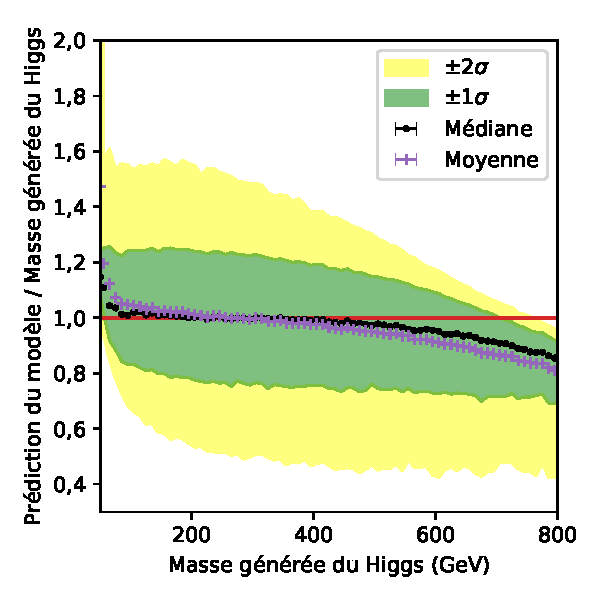
\includegraphics[width=\textwidth]{\PhDthesisdir/plots_and_images/my_plots/ML/from_ML_plots/trained_NNs_FastSim/DeepTau-inclusive/PuppiMET_with_METcov_j1j2jr_Nnu_Npu/model_response-NN-ADAM_glorot_uniform-activation-elu-batch_size-2048-mape-Adadelta-u-inclusive-3-layers-1000-neurons.pdf}

\caption{Réponse du modèle A.}
\label{subfig-reponse_model_A}
\end{figure}
\end{minipage}
\end{figure}
\begin{figure}[p]
\centering

\subcaptionbox{Réponse du modèle B.\label{subfig-reponse_model_B}}[.45\textwidth]
{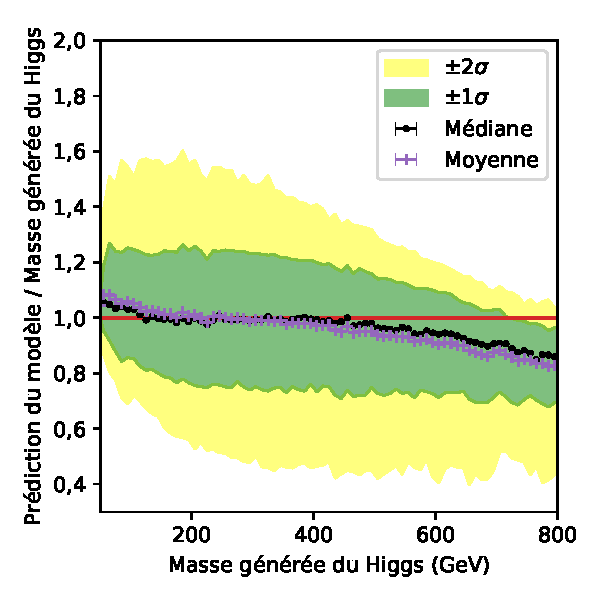
\includegraphics[width=.45\textwidth]{\PhDthesisdir/plots_and_images/my_plots/ML/from_ML_plots/trained_NNs_FastSim/DeepTau-inclusive/PuppiMET_with_METcov_j1j2jr_Nnu_Npu/model_response-NN-ADAM_glorot_uniform-activation-softplus-batch_size-2048-mape-Adadelta-u-inclusive-3-layers-1000-neurons.pdf}\vspace{-.5\baselineskip}}
\hfill
\subcaptionbox{Réponse du modèle C.\label{subfig-reponse_model_C}}[.45\textwidth]
{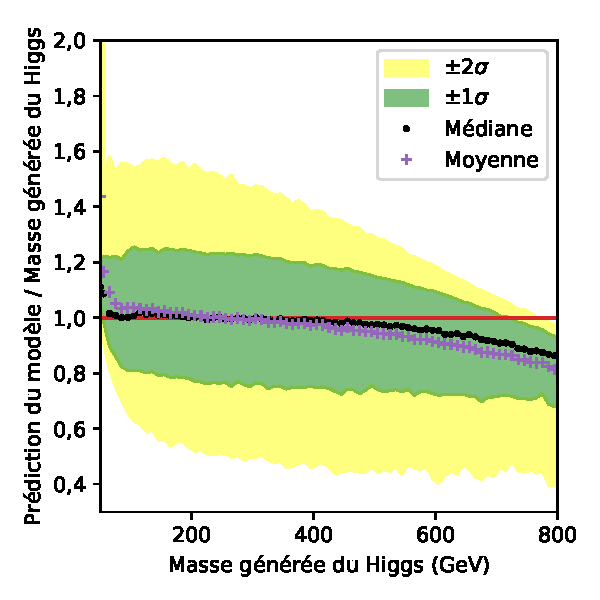
\includegraphics[width=.45\textwidth]{\PhDthesisdir/plots_and_images/my_plots/ML/from_ML_plots/trained_NNs_FastSim/DeepTau-inclusive/PuppiMET_with_METcov_j1j2jr_Nnu_Npu/model_response-NN-activation-selu-batch_size-2048-mape-Adam-n-inclusive-3-layers-1000-neurons.pdf}\vspace{-.5\baselineskip}}

\subcaptionbox{Réponse du modèle D.\label{subfig-reponse_model_D}}[.45\textwidth]
{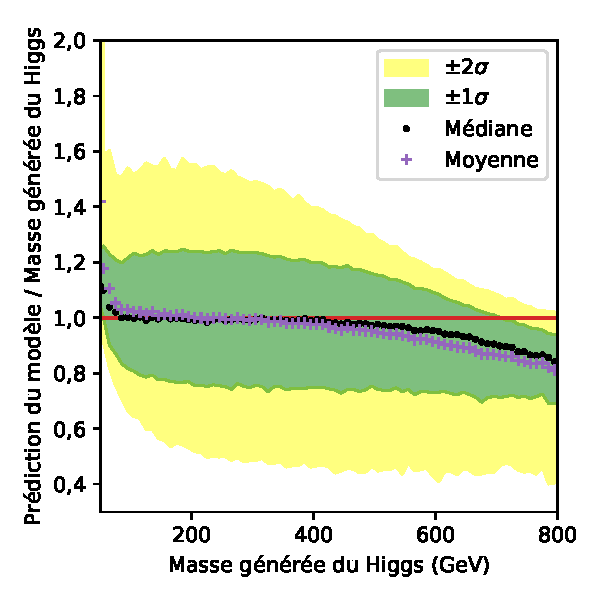
\includegraphics[width=.45\textwidth]{\PhDthesisdir/plots_and_images/my_plots/ML/from_ML_plots/trained_NNs_FastSim/DeepTau-inclusive/PuppiMET_with_METcov_j1j2jr_Nnu_Npu/model_response-NN-activation-relu-batch_size-2048-mape-Adam-gu-inclusive-3-layers-1400-neurons.pdf}\vspace{-.5\baselineskip}}
\hfill
\subcaptionbox{Réponse du modèle E.\label{subfig-reponse_model_E}}[.45\textwidth]
{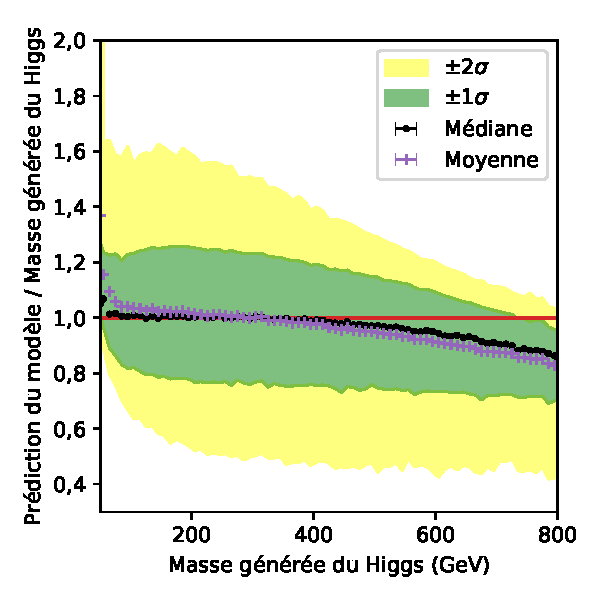
\includegraphics[width=.45\textwidth]{\PhDthesisdir/plots_and_images/my_plots/ML/from_ML_plots/trained_NNs_FastSim/DeepTau-inclusive/PuppiMET_with_METcov_j1j2jr_Nnu_Npu/model_response-NN-activation-relu-batch_size-2048-mape-Adam-gn-inclusive-4-layers-200-neurons.pdf}\vspace{-.5\baselineskip}}

\subcaptionbox{Réponse du modèle F.\label{subfig-reponse_model_F}}[.45\textwidth]
{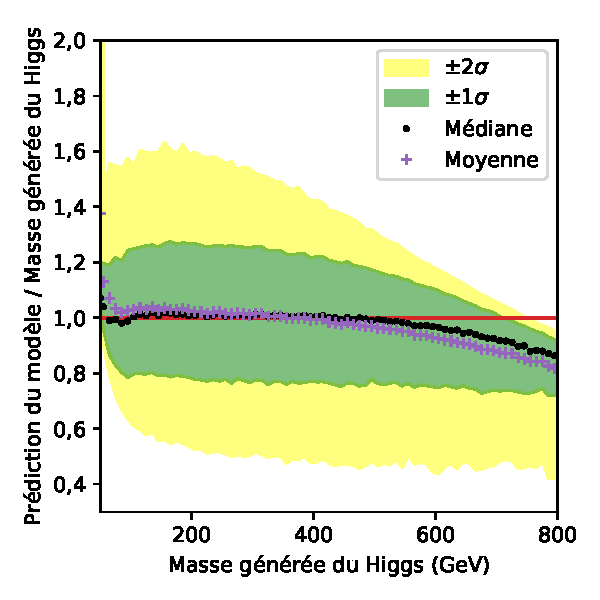
\includegraphics[width=.45\textwidth]{\PhDthesisdir/plots_and_images/my_plots/ML/from_ML_plots/trained_NNs_FastSim/DeepTau-inclusive/PuppiMET_with_METcov_j1j2jr_Nnu_Npu/model_response-NN-activation-elu-batch_size-2048-mape-Adam-gu-inclusive-4-layers-1000-neurons.pdf}\vspace{-.5\baselineskip}}
\hfill
\subcaptionbox{Réponse du modèle G.\label{subfig-reponse_model_G}}[.45\textwidth]
{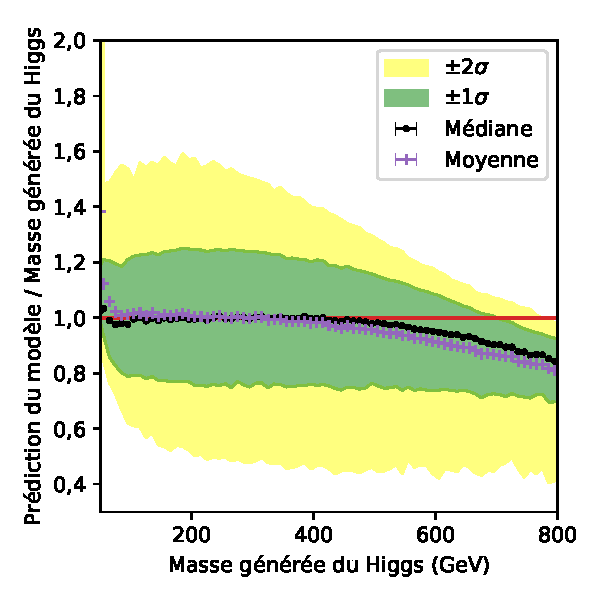
\includegraphics[width=.45\textwidth]{\PhDthesisdir/plots_and_images/my_plots/ML/from_ML_plots/trained_NNs_FastSim/DeepTau-inclusive/PuppiMET_with_METcov_j1j2jr_Nnu_Npu/model_response-NN-activation-softplus-batch_size-2048-mape-Adam-gu-inclusive-4-layers-1400-neurons.pdf}\vspace{-.5\baselineskip}}

\caption{Réponse des modèles B à G.}
\label{fig-reponse_model_B_to_G}
\end{figure}
\par
La même procédure appliquée à tous les modèles entraînés mène à une liste
ne contenant que des DNNs,
utilisant majoritairement les 27 variables d'entrée,
tous entraînés par Adam avec comme fonction de coût \LossMAPE,
ce qui confirme que nos choix d'hyper-paramètres précédents sont pertinents.
\par
Aucun modèle avec $N_L\in\set{2,5}$ n'est sélectionné.
Pour 4 modèles, $N_L=3$.
Le nombre de neurones par couche cachée est de \num{1000} pour 4 modèles sur 7, dont 3 sur les 4 avec $N_L=3$.
Le WI le plus représenté est Glorot uniforme (5/7).
Les FA sont disparates, chacune apparaissant une ou deux fois dans la sélection.
\par
Chacun de ces modèles présente une réponse proche de 1 entre \num{70} et \SI{400}{\GeV} avec une résolution à $\pm1\sigma$ de l'ordre de \SI{22}{\%} à basse masse et \SI{10}{\%} à haute masse.
Le modèle F conserve une réponse proche de 1 jusqu'à environ \SI{500}{\GeV}, cependant se résolution à basse masse en légèrement dégradée par rapport aux autres modèles.
Le modèle B a des hyper-paramètres \og consensus \fg,
\ie\ que chacune des valeurs de ses hyper-paramètres correspond à la valeur la plus représentée dans la sélection.
C'est à partir de ce modèle que nous avons choisi de continuer notre étude.
Les hyper-paramètres sélectionnés sont donnés dans le tableau~\ref{tab-compare_DNN_to_BARTSCHI201929}
avec une comparaison à ceux utilisés par \citeauthor{BARTSCHI201929}~\cite{BARTSCHI201929}.
\begin{table}[h]
\centering
\begin{tabular}{lcc}
\toprule
Hyper-paramètre & Notre DNN & DNN de \citeauthor{BARTSCHI201929}~\cite{BARTSCHI201929}\\
\midrule
Nombre de couches cachées $N_L$ & 3 & 4 \\
Neurones par couche cachée $N_N$ & 1000 & 200 \\
Fonction d'activation & Softplus & ReLU \\
Algorithme d'optimisation & Adam & Adam \\
Fonction de coût & \LossMAPE & \LossMSE \\
Initiation des poids & \og Glorot Uniforme \fg~\cite{glorot} & ? \\
Nombre d'entrées & 27 (voir section~\ref{chapter-ML-section-evt_gen-inputs}) & 17 (voir~\cite{BARTSCHI201929}) \\
\bottomrule
\end{tabular}
\caption[Comparaison de nos hyper-paramètres à ceux de \citeauthor{BARTSCHI201929}.]{Comparaison de nos hyper-paramètres à ceux de \citeauthor{BARTSCHI201929}. Le mode d'initiation des poids utilisé par \citeauthor{BARTSCHI201929} n'est pas donné dans leur article.}
\label{tab-compare_DNN_to_BARTSCHI201929}
\end{table}
%\begin{itemize}
%\item 3 couches cachées;
%\item \num{1000} neurones par couche cachée;
%\item fonction d'activation Softplus, $x\mapsto\ln(1+\eexp{x})$;
%\item algorithme d'optimisation Adam, présenté en section~\ref{chapter-ML-section-DNN-training-optimizers};
%\item fonction de coût MAPE, définie équation~\eqref{eq-loss_MAPE};
%\item initiation des poids selon le mode \og Glorot Uniforme \fg~\cite{glorot};
%\item la liste des 27 variables d'entrée égale à celle donnée en section~\ref{chapter-ML-section-evt_gen-inputs}.
%\end{itemize}
%En comparaison, le DNN de \citeauthor{BARTSCHI201929}~\cite{BARTSCHI201929} a pour hyper-paramètres:
%\begin{itemize}
%\item 4 couches cachées;
%\item \num{200} neurones par couche cachée;
%\item fonction d'activation ReLU y compris pour la couche de sortie;
%\item algorithme d'optimisation Adam;
%\item fonction de coût MSE, définie équation~\eqref{eq-loss_MSE};
%\item 17 variables d'entrée:
%\begin{itemize}
%\item les impulsions, énergies et masses invariantes de $L_1$ et $L_2$:\\
%$\pT^{L_1}$, $\eta^{L_1}$, $\phi^{L_1}$, $E^{L_1}$, $\minv^{L_1}$,
%$\pT^{L_2}$, $\eta^{L_2}$, $\phi^{L_2}$, $E^{L_2}$, $\minv^{L_2}$;
%\item l'énergie transverse manquante:\\
%\MET, $\phi^{\MET}$;
%\item la masse colinéaire du système di-\tau, $m_\text{coll}$, définie dans~\cite{BARTSCHI201929};
%\item 4 booléens donnant le type de canal (hadronique, semi-leptonique ou leptonique).
%\end{itemize}
%\end{itemize}

%\includegraphics[width=.45\textwidth]{\PhDthesisdir/plots_and_images/my_plots/ML/from_ML_plots/global_comparisons/DNN_structures_reduced-full_mape.pdf}
%\includegraphics[width=.45\textwidth]{\PhDthesisdir/plots_and_images/my_plots/ML/from_ML_plots/global_comparisons/DNN_structures_all-full_mape.pdf}
%several possibilities, but the loss mass region contains the Z boson and is important
%\includegraphics[width=.45\textwidth]{\PhDthesisdir/plots_and_images/my_plots/ML/from_ML_plots/global_comparisons/DNN_structures_reduced-low_mape.pdf}
%\includegraphics[width=.45\textwidth]{\PhDthesisdir/plots_and_images/my_plots/ML/from_ML_plots/global_comparisons/DNN_structures_all-low_mape.pdf}
%2x900 and 5x600 seem to be the best options, check the low mass resolution
%\includegraphics[width=.45\textwidth]{\PhDthesisdir/plots_and_images/my_plots/ML/from_ML_plots/global_comparisons/DNN_structures_reduced-low_1sig_width.pdf}
%\includegraphics[width=.45\textwidth]{\PhDthesisdir/plots_and_images/my_plots/ML/from_ML_plots/global_comparisons/DNN_structures_all-low_1sig_width.pdf}
%5x600 seems good, check the low mass \textbf{calibrated} resolution
%\includegraphics[width=.45\textwidth]{\PhDthesisdir/plots_and_images/my_plots/ML/from_ML_plots/global_comparisons/DNN_structures_reduced-low_1sig_calibr_width.pdf}
%\includegraphics[width=.45\textwidth]{\PhDthesisdir/plots_and_images/my_plots/ML/from_ML_plots/global_comparisons/DNN_structures_all-low_1sig_calibr_width.pdf}
%and in the medium mass region we have
%\includegraphics[width=.45\textwidth]{\PhDthesisdir/plots_and_images/my_plots/ML/from_ML_plots/global_comparisons/DNN_structures_reduced-medium_mape.pdf}
%\includegraphics[width=.45\textwidth]{\PhDthesisdir/plots_and_images/my_plots/ML/from_ML_plots/global_comparisons/DNN_structures_all-medium_mape.pdf}
%3x1000 is the best compromise we found